\documentclass[12pt,a4paper]{article}
\makeatletter\def\input@path{{report/}}\makeatother
\usepackage{assignment_format}
\usepackage{longtable,calc,listings,etoolbox}
\providecommand{\tightlist}{\setlength{\itemsep}{0pt}\setlength{\parskip}{0pt}}
\providecommand{\passthrough}[1]{#1}
\newcounter{none}
\lstset{basicstyle=\ttfamily\scriptsize,breaklines=true,columns=fullflexible,
 keepspaces=true,showstringspaces=false,frame=single,rulecolor=\color{accent!40},
 backgroundcolor=\color{black!2},numbers=left,numberstyle=\tiny,numbersep=5pt,
 xleftmargin=8pt,framexleftmargin=5pt,aboveskip=8pt,belowskip=8pt}
\setlength{\LTpre}{5pt}\setlength{\LTpost}{5pt}
\AtBeginEnvironment{longtable}{\small\linespread{1.05}\selectfont}
\DeclareUnicodeCharacter{2212}{\ensuremath{-}}
\DeclareUnicodeCharacter{2264}{\ensuremath{\leq}}
\DeclareUnicodeCharacter{2265}{\ensuremath{\geq}}
\DeclareUnicodeCharacter{03B5}{\ensuremath{\epsilon}}
\DeclareUnicodeCharacter{03B1}{\ensuremath{\alpha}}
\DeclareUnicodeCharacter{03B3}{\ensuremath{\gamma}}
\DeclareUnicodeCharacter{00D7}{\ensuremath{\times}}
\DeclareUnicodeCharacter{2192}{\ensuremath{\rightarrow}}
\DeclareUnicodeCharacter{00B1}{\ensuremath{\pm}}
\hypersetup{pdftitle={BÁO CÁO THỰC HÀNH AGENT 02},pdfauthor={Nguyễn Nam Hải -- B23DCCN277}}
\begin{document}
\hypersetup{pageanchor=false}
\begin{titlepage}
    \begin{tikzpicture}[remember picture,overlay]
        \draw[line width=2.2pt,color=black]
            ([xshift=15mm,yshift=-15mm]current page.north west) rectangle
            ([xshift=-15mm,yshift=15mm]current page.south east);
        \draw[line width=0.8pt,color=black]
            ([xshift=17.5mm,yshift=-17.5mm]current page.north west) rectangle
            ([xshift=-17.5mm,yshift=17.5mm]current page.south east);
    \end{tikzpicture}
    \centering
    \vspace*{0.2cm}
    {\large\textbf{HỌC VIỆN CÔNG NGHỆ BƯU CHÍNH VIỄN THÔNG}}\\[0.25cm]
    {\large\textbf{KHOA CÔNG NGHỆ THÔNG TIN 1}}\\[0.2cm]
    \rule{5cm}{1pt}\\[0.7cm]
    
\includegraphics[width=3.4cm,height=4.2cm,keepaspectratio]{assets/logo_ptit.png}\\[0.8cm]
    {\Large\textbf{BÁO CÁO THỰC HÀNH AGENT 02}}\\[0.35cm]
    {\large\textbf{MÔN HỌC: PHÁT TRIỂN CÁC HỆ THỐNG THÔNG MINH}}\\[0.55cm]
    {\large\textbf{REINFORCEMENT LEARNING VÀ RULE-BASED AGENTS}}\\[0.25cm]
    \begin{flushleft}
    \hspace*{1.1cm}
    \begin{tabular}{p{5.2cm}p{0.3cm}l}
        \textbf{Giảng viên hướng dẫn} & : & \textbf{PGS.TS. Trần Đình Quế}\\[0.25cm]
        \textbf{Lớp} & : & \textbf{D23CTPM01}\\[0.25cm]
        \textbf{Nhóm học phần} & : & \textbf{CT01}\\[0.25cm]
        \textbf{Sinh viên thực hiện} & : & \textbf{Nguyễn Nam Hải}\\[0.25cm]
        \textbf{Mã sinh viên} & : & \textbf{B23DCCN277}\\[0.25cm]
    \end{tabular}
    \end{flushleft}
    \vfill
    {\large\textbf{Hà Nội -- Năm 2026}}
    \vspace*{0.3cm}
\end{titlepage}
\hypersetup{pageanchor=true}

\pagenumbering{roman}
\setcounter{tocdepth}{2}
{\linespread{1.0}\selectfont\tableofcontents}
\clearpage\listoffigures\clearpage
\section*{DANH MỤC THUẬT NGỮ}
\addcontentsline{toc}{section}{Danh mục thuật ngữ}
\begin{tabularx}{\linewidth}{p{2.5cm}X}
\toprule
MAS & Multi-Agent System -- Hệ đa tác tử\\
LLM & Large Language Model -- Mô hình ngôn ngữ lớn\\
RL / MARL & Reinforcement Learning / Multi-Agent RL\\
MDP / POMDP & Quá trình quyết định Markov / quan sát không đầy đủ\\
TD / Q & Sai phân thời gian / Giá trị hành động\\
DP & Dynamic Programming -- Quy hoạch động\\
OOD & Out-of-distribution -- Ngoài phân phối/ngoài miền\\
PEAS & Performance, Environment, Actuators, Sensors\\
DAG & Directed Acyclic Graph -- Đồ thị có hướng không chu trình\\
SD / CI & Độ lệch chuẩn mẫu / Khoảng tin cậy\\
P50 / P95 & Phân vị 50 / 95 của thời gian phản hồi\\
TTL & Time to Live -- Giới hạn độ mới của dữ liệu\\
\bottomrule
\end{tabularx}
\vspace{8mm}
\begin{academicbox}{Quy ước đọc báo cáo}
Dữ liệu thực hành là tổng hợp hoặc mô phỏng. Số đo được lấy từ mã đã chạy và lưu kèm; phép tính lý thuyết và đề xuất chưa thực hiện được gọi rõ. Thông tin bìa, logo và phong cách trình bày kế thừa báo cáo trước. Ngày hoàn thiện: 28/10/2026.
\end{academicbox}
\clearpage\pagenumbering{arabic}\setcounter{page}{1}
\section{Giới thiệu và mục tiêu thí
nghiệm}\label{giux1edbi-thiux1ec7u-vuxe0-mux1ee5c-tiuxeau-thuxed-nghiux1ec7m}

Laboratory Experiment 02 yêu cầu triển khai và so sánh
reinforcement-learning-based agent với rule-based agent trong thị trường
thương mại điện tử đơn giản. Báo cáo hoàn thành thí nghiệm A--E, giải đủ
mười câu hỏi, triển khai biến đổi môi trường, thử đồng học và xây dựng
một agent mốc tốt hơn bằng quy hoạch động. Các kết quả trong bảng và
hình được tạo từ mã chạy thật; dữ liệu thị trường là mô phỏng, không
phải số liệu kinh doanh thực tế. \cite{lab}

Theo đề, hạn nộp là 23:30 thứ Năm ngày 29/10/2026. Tên tệp theo quy ước
và thông tin kế thừa từ bài trước là
\passthrough{\lstinline!agent02\_CT\_04\_hainn.pdf!}. Bìa sử dụng PTIT,
lớp D23CTPM01, nhóm học phần CT01, Nguyễn Nam Hải, mã B23DCCN277 và
giảng viên PGS.TS. Trần Đình Quế. Các thông tin này lấy từ báo cáo trước
trong workspace.

Có ba mục tiêu đánh giá riêng: hành vi học thay đổi thế nào qua tương
tác; policy đóng băng đạt lợi nhuận bao nhiêu; và kết quả có ổn định khi
thay seed hoặc tham số môi trường không. Một đường reward tăng không tự
trả lời hai câu sau. Báo cáo vì thế tách training, evaluation, fair
policy comparison và robustness.

\section{Mô tả môi trường và hai tác
tử}\label{muxf4-tux1ea3-muxf4i-trux1b0ux1eddng-vuxe0-hai-tuxe1c-tux1eed}

\subsection{Mô hình thị
trường}\label{muxf4-huxecnh-thux1ecb-trux1b0ux1eddng}

Hai cửa hàng A và B chọn đồng thời hành động \(a_i\in\{0,1\}\), lần lượt
là không giảm và giảm giá. Không agent nào được nhìn hành động hiện tại
của đối thủ trước khi chọn. Mỗi bên quan sát nhu cầu \(d\in\{0,1\}\) và
hành động trước của đối thủ. Không gian quan sát cục bộ có bốn phần tử
và hai hành động nên bảng Q tham chiếu có tám giá trị.

Nhu cầu thấp có 10 khách hàng tiềm năng, nhu cầu cao có 20. Xác suất
chuyển đổi cho agent \(i\) là:

\[p_i=\operatorname{clip}(0.30+0.25d+0.15a_i-0.10a_{-i},0.05,0.95).\]

Doanh số \(S_i\sim\operatorname{Binomial}(N_d,p_i)\); giá gốc \(P=10\),
unit cost \(C=5\), discount fraction \(\delta=0.20\); reward:

\[r_i=S_i\,[P(1-\delta a_i)-C].\]

Nhu cầu tiếp theo lấy đều độc lập; hành động hiện tại trở thành lịch sử
của bước sau. Sales hai cửa hàng được lấy mẫu riêng có điều kiện theo
nhu cầu và hành động, không có ràng buộc tổng sales không vượt một nhóm
khách hàng duy nhất. Vì vậy đây là mô hình tương tác cạnh tranh có tổng
lợi ích thay đổi, không phải mô phỏng thị phần đầy đủ hoặc trò chơi tổng
bằng không.

\subsection{Agent A: Q-learning}\label{agent-a-q-learning}

Agent A dùng bảng \(Q[d,c,a]\). Trong training, nó khám phá theo
epsilon-greedy và cập nhật:

\[Q(s,a)\leftarrow Q(s,a)+\alpha[r+\gamma\max_{a'}Q(s',a')-Q(s,a)].\]

Bước cuối dùng target \(r\) vì được coi là terminal trong protocol tham
chiếu. Evaluation dùng argmax xác định, epsilon 0 và không gọi learn.
Phân xử hòa trong evaluation chọn action 0; training phá hòa ngẫu nhiên.
Quy ước này được công bố vì các policy snapshot cần cho cùng kết quả khi
chạy lại.

\subsection{Agent B: luật cố
định}\label{agent-b-luux1eadt-cux1ed1-ux111ux1ecbnh}

Luật là \(\pi_B(d,c)=1\) khi \(d=1\) và \(c=1\), còn lại bằng 0. Khi nhu
cầu thấp, B không giảm. Khi nhu cầu cao, B chỉ giảm nếu A đã giảm ở bước
trước. B không cập nhật từ reward và không có bảng Q. Tuy nhiên, hành
động của B vẫn phụ thuộc quan sát và có thể thay đổi theo thời gian;
không học không đồng nghĩa luôn có cùng một hành động.

\subsection{Hai vấn đề trạng thái cần lưu
ý}\label{hai-vux1ea5n-ux111ux1ec1-trux1ea1ng-thuxe1i-cux1ea7n-lux1b0u-uxfd}

Quan sát cục bộ của A thiếu hành động trước của chính A, trong khi luật
B sử dụng đúng bit đó. Với cùng \((d=1,c_B=0)\), B có thể chọn 0 hoặc 1
tùy hành động trước của A. Vì vậy quan sát tham chiếu không đảm bảo
Markov đối với learner. Mã giữ nó để so sánh đúng baseline, nhưng báo
cáo không áp một định lý MDP đầy đủ lên biểu diễn này.

Episode có 20 bước và target terminal ở cuối, nhưng bảng Q không chứa
thời gian. Một quan sát ở đầu kỳ và cuối kỳ nhận các target có độ dài
tương lai khác nhau. Đây là vấn đề hữu hạn chân trời bị gộp trong một
bảng. Agent cải tiến dùng trạng thái đầy đủ và chỉ số thời gian, được
trình bày ở Câu 10.

\section{Mã nguồn và thay đổi so với tài liệu tham
chiếu}\label{muxe3-nguux1ed3n-vuxe0-thay-ux111ux1ed5i-so-vux1edbi-tuxe0i-liux1ec7u-tham-chiux1ebfu}

Tệp \passthrough{\lstinline!assignment/reference\_agent02.py!} là bản
sao nguyên văn chương trình được cung cấp trong
\passthrough{\lstinline!agent02\_code.tex!}, lưu riêng để đối chiếu. Tệp
\passthrough{\lstinline!assignment/agent02\_experiment.py!} triển khai
môi trường, Q-learning, luật, train, evaluate và chương trình xuất dữ
liệu. Mã gốc được chạy thêm riêng cho seed 42; kết quả lưu với tiền tố
\passthrough{\lstinline!reference\_original\_42!}.

Các thay đổi được công bố rõ: tách stream random nhu cầu, sales và agent
bằng SeedSequence; đánh giá vector hóa theo episode với common random
numbers; dùng cùng opponent cho so sánh policy; chạy toàn bộ cấu hình
trên năm seed; xuất learning curves cho cả alpha và epsilon; bổ sung
discount 40\%, self-play và oracle DP. Quy luật phân phối nhu cầu,
conversion, sales và margin được giữ nguyên cho baseline.

Tách RNG không tạo ra cùng chuỗi số ngẫu nhiên như chương trình gốc dù
cùng seed số học. Vì vậy kết quả baseline 42 của bản mở rộng
\textbf{không được gọi là tái lập bit-for-bit} của code gốc. Đó là một
thực nghiệm cùng mô hình phân phối với protocol random rõ hơn. Sự khác
biệt này còn được kiểm tra bằng việc chạy bản gốc riêng và đưa cả hai
vào phụ lục số liệu.

Common random numbers trong evaluation được tạo bằng cùng demand tape và
cùng tensor uniform Bernoulli cho mọi focal policy trên một seed. Nếu
xác suất chuyển đổi tăng, cùng uniform cho phép so sánh có ghép cặp; số
lượng sales vẫn có phân phối binomial đúng. Khi policy làm lịch sử khác
đi, reward có thể khác, nhưng nhiễu đầu vào được kiểm soát tốt hơn so
với hai lần chạy hoàn toàn độc lập.

\section{Thiết lập thực nghiệm và
protocol}\label{thiux1ebft-lux1eadp-thux1ef1c-nghiux1ec7m-vuxe0-protocol}

{\def\LTcaptype{none} % do not increment counter
\begin{longtable}[]{@{}ll@{}}
\toprule\noalign{}
Tham số & Giá trị \\
\midrule\noalign{}
\endhead
\bottomrule\noalign{}
\endlastfoot
Training episodes & 5.000 mỗi lần train \\
Steps/episode & 20 \\
Evaluation episodes & 500 \\
Evaluation steps & 10.000 mỗi cặp policy/seed \\
Gamma & 0.90 \\
Alpha baseline & 0.10 \\
Epsilon baseline & max(0.02, 0.20 × 0.995\^{}episode\_index) \\
Alpha sensitivity & 0.01, 0.10, 0.50 \\
Epsilon sensitivity & Schedule baseline; fixed 0.05; fixed 0.30 \\
Training seeds & 11, 22, 33, 44, 55; run minh họa riêng seed 42 \\
Evaluation seeds & 800000 + training seed \\
Evaluation riêng seed 42 & 500042 \\
Self-play evaluation & 900000 + training seed \\
Discount robustness & 40\%, giữ các tham số còn lại \\
\end{longtable}
}

Năm seed được dùng nhất quán cho mỗi cấu hình alpha/epsilon. Mỗi cấu
hình có 500.000 bước training cộng 50.000 bước evaluation. Toàn bộ
baseline và mở rộng có 36 lượt training của chương trình mở rộng: 25
lượt sensitivity, một lượt minh họa seed 42, năm lượt retrain discount
40\% và năm lượt self-play. Tính theo môi trường là 3.600.000 bước
training; các lượt self-play cập nhật hai Q-table mỗi bước.

Đơn vị reward trong báo cáo là đơn vị lợi nhuận của mô hình, không được
gán thành VND hoặc USD vì đề không quy định tiền tệ. Reward trung bình
tính bằng tổng profit chia tổng bước. Standard deviation trong bảng cấu
hình là sample SD trên năm \textbf{run means}, không phải SD của toàn bộ
từng bước. SD từng episode được lưu riêng trong summary và không thay
thế biến động giữa seed.

Khoảng tin cậy minh họa cho mean qua năm seed dùng
\(t_{0.975,4}=2.776\), tức \(\bar x\pm2.776s/\sqrt5\). Với chỉ năm seed
và policy phân phối có thể không chuẩn, khoảng này có tính xấp xỉ và dễ
rộng. Báo cáo không dùng nó như bằng chứng chắc chắn về mọi môi trường
hoặc mọi lần train.

\section{Thí nghiệm A --- Baseline và policy đã
học}\label{thuxed-nghiux1ec7m-a-baseline-vuxe0-policy-ux111uxe3-hux1ecdc}

Lượt minh họa mở rộng seed 42 cho focal RL tổng reward 255591, trung
bình 25.5591 trên 10.000 bước; opponent rule tổng 246856, trung bình
24.6856. RL không giảm 1849 lần và giảm 8151 lần, tức 81.51\%; opponent
giảm 38.53\%. Đây là một policy seed cụ thể có chất lượng thấp so với
mốc không giảm giá, không phải con số đại diện duy nhất cho Q-learning.

Bảng Q đầy đủ và policy ở bốn trạng thái được sinh từ
\passthrough{\lstinline!baseline\_42\_q.npy!}, hiển thị ở phần số liệu
tự động cùng heatmap. Vì reward discounted dài hạn có thể lớn hơn reward
tức thời, độ lớn Q không được so trực tiếp với profit mỗi bước. Việc Q
lớn chưa chứng minh greedy action đúng; phải đánh giá policy và đối
chiếu oracle.

Ở năm seed dùng cho so sánh chính, baseline RL đạt mean 34.0997, SD
1.3678. Hai seed 22 và 33 học policy còn giảm giá đáng kể, các seed 11,
44 và 55 đạt hành vi không giảm ở các trạng thái đã gặp trong
evaluation. Chênh lệch lớn giữa seed 42 và nhóm năm seed là bằng chứng
rất rõ về rủi ro kết luận từ một lần chạy.

Cũng cần lưu ý reward đối thủ trong cùng trận không phải baseline tách
biệt cùng đối thủ. Khi A giảm, B có thể phản ứng; hai bên không có cùng
chuỗi quyết định. Vì vậy việc RL 25.56 cao hơn opponent 24.69 ở seed 42
không chứng minh RL tốt hơn mọi rule policy. Thí nghiệm E mới so sánh
các focal policy dưới cùng opponent cố định.

\section{Thí nghiệm B --- Quá trình
học}\label{thuxed-nghiux1ec7m-b-quuxe1-truxecnh-hux1ecdc}

Learning curve dùng reward/step mỗi episode, làm trơn bằng trung bình
trượt 100 episode. Trục x gắn với cuối cửa sổ; hình tổng hợp thể hiện
mean và vùng ±1 SD trên năm seed. Đó là cửa sổ trượt có chồng lấn, vì
vậy các điểm liên tiếp không độc lập thống kê. Số liệu episode thô vẫn
được giữ trong CSV.

Baseline có trung bình 500 episode đầu là 32.8595 và 500 episode cuối là
33.6718. Quan sát này phù hợp với việc policy cải thiện một phần trong
training, nhưng mức tăng khoảng 0.8124 không chứng minh hội tụ hoặc tối
ưu. Các đường còn dao động do nhu cầu, sales, khám phá và cập nhật Q.

Nếu nhìn cả training mean 33.6513 và frozen evaluation mean 34.0997,
evaluation cao hơn trong nhóm seed này. Một giải thích phù hợp là tắt
khám phá giảm chi phí thử hành động. Tuy nhiên, không nên quy mọi chênh
lệch cho epsilon vì evaluation dùng dữ liệu khác và policy cuối chỉ là
một snapshot. Các giới hạn về aliasing và thời gian vẫn tồn tại khi
epsilon bằng 0.

Để nghiên cứu hội tụ sâu hơn, cần lưu Q qua các checkpoint, đo thay đổi
policy, visit counts và regret so với oracle. Bộ bài hiện đã cung cấp
bảng Q cuối, learning curve và nhiều seed; chưa thực hiện chuỗi
checkpoint lớn nên không đưa kết luận về tốc độ hội tụ chính xác.

\section{Thí nghiệm C --- Learning
rate}\label{thuxed-nghiux1ec7m-c-learning-rate}

Ba alpha 0.01, 0.10 và 0.50 giữ nguyên gamma, số episode và epsilon
schedule. Mean đánh giá lần lượt 33.6484, 34.0997 và 31.9533; SD giữa
seed lần lượt 2.1286, 1.3678 và 4.1613. Trong những run đã đo, alpha
0.10 có mean cao và biến động thấp hơn hai lựa chọn còn lại.

Alpha 0.01 tăng training từ 30.9924 ở 500 episode đầu lên 33.7541 ở 500
episode cuối, cho thấy việc cập nhật chậm có thể cần nhiều tương tác.
Alpha 0.50 có SD đánh giá lớn, phù hợp với độ nhạy cao trước nhiễu
reward và target. Nhưng dữ liệu này không đủ để nói learning rate 0.50
luôn gây bất ổn trong mọi môi trường.

Một điểm kỹ thuật là target terminal giảm mạnh ở cuối mỗi episode. Alpha
lớn đưa trọng số lớn hơn cho các mẫu đó, trong khi state không chứa thời
gian. Do vậy tác động alpha bị trộn với thiết kế biểu diễn. Muốn tách
nguyên nhân, cần thêm ablation Q có chỉ số thời gian trên cùng alpha;
đây là thí nghiệm được đề xuất chứ chưa được báo như đã chạy.

\section{Thí nghiệm D --- Khám
phá}\label{thuxed-nghiux1ec7m-d-khuxe1m-phuxe1}

Schedule baseline, epsilon cố định 0.05 và cố định 0.30 cho mean
evaluation lần lượt 34.0997, 33.3973 và 31.4300; SD lần lượt 1.3678,
1.6126 và 3.9272. Mean training tương ứng 33.6513, 32.9458 và 30.8822.
Cấu hình khám phá cao không có lợi trong bộ run hiện tại.

Mức epsilon 0.30 không có nghĩa 30\% bước chắc chắn chọn hành động không
greedy. Với hai action, nhánh ngẫu nhiên vẫn có xác suất chọn greedy.
Ngoài ra, tỷ lệ discount cuối còn phụ thuộc policy đã học, nên discount
rate evaluation không bằng epsilon training. Báo cáo ghi riêng các đại
lượng trong CSV để tránh đồng nhất chúng.

Tắt khám phá trong evaluation cần thiết để đo policy greedy, nhưng không
sửa một bảng Q đã học sai. Đối với seed học ra lựa chọn discount không
tốt, epsilon 0 làm lựa chọn đó lặp nhất quán. Vì vậy thiết kế khám phá
cần được đánh giá bằng cả hiệu năng trong training, chất lượng cuối và
biến động giữa seed.

\section{Thí nghiệm E --- So sánh policy công
bằng}\label{thuxed-nghiux1ec7m-e-so-suxe1nh-policy-cuxf4ng-bux1eb1ng}

Focal policies gồm Q-learning, rule tham chiếu, luôn không giảm, luôn
giảm và DP. Tất cả được đánh giá với cùng rule opponent, cùng seeds và
cùng random tapes. Không cập nhật bất kỳ Q nào. Đây là phép so sánh phù
hợp hơn việc chỉ đặt reward hai bên của một trận cạnh nhau.

Rule và never-discount đạt cùng hành vi khi cả hai lịch sử khởi đầu bằng
0. DP cũng chọn không giảm ở mọi state/time với tham số mặc định. Do
cùng action và tape, ba hàng này có số đo giống hệt nhau từng seed. Mean
khoảng 35.1295 không phải 35 đúng tuyệt đối; 35 là kỳ vọng lý thuyết, số
đo hữu hạn có nhiễu.

RL baseline đạt 34.0997; mức kém hơn rule trên nhóm seed này khoảng
1.0298 lợi nhuận/step. Đây là kết quả trong môi trường tham chiếu. Nó
không chứng minh rule tốt hơn RL ở mọi bài toán; thay đổi conversion,
chi phí, đối thủ hoặc state có thể tạo kết quả khác. Điều có thể kết
luận là baseline Q-learning hiện tại chưa vượt được một policy xác định
rất đơn giản trong mô hình này.

\section{Trả lời đầy đủ mười câu
hỏi}\label{trux1ea3-lux1eddi-ux111ux1ea7y-ux111ux1ee7-mux1b0ux1eddi-cuxe2u-hux1ecfi}

\subsection{Câu 1 --- Mô hình tác tử và môi
trường}\label{cuxe2u-1-muxf4-huxecnh-tuxe1c-tux1eed-vuxe0-muxf4i-trux1b0ux1eddng}

Hai tác tử là hai cửa hàng chọn giảm giá. Môi trường gồm nhu cầu, lịch
sử hành động, quá trình sales và quy tắc profit. Observation mỗi agent
là \((d,c)\); action gồm 0/1; reward là lợi nhuận đã trừ unit cost sau
giảm giá; chuyển tiếp cập nhật lịch sử và sinh nhu cầu mới. Bốn
observation kết hợp hai action tạo tám mục Q.

Đây là MAS vì reward của mỗi bên phụ thuộc hành động bên kia qua hệ số
\(-0.10a_{-i}\) và quan sát tương lai chứa hành động đối thủ. Hai policy
có mục tiêu lợi nhuận riêng và quyết định tương tác. Không có thông điệp
chat vẫn có thể là MAS: môi trường chung là kênh tương tác. Khi giữ
opponent cố định, có thể phân tích learner như bài điều khiển trong một
môi trường hiệu dụng, nhưng bản chất hệ gốc vẫn có hai tác tử.

Phân biệt observation với full state là cần thiết. Trạng thái đầy đủ
\(x=(d,a_{t-1}^A,a_{t-1}^B)\) có tám tổ hợp, thêm thời gian nếu hữu hạn
chân trời. Observation tham chiếu chỉ là một phép chiếu của full state.
Nêu điều này giúp tránh gọi bốn observation là một MDP đầy đủ mà chưa
kiểm giả định.

\subsection{Câu 2 --- Quyết định học và theo
luật}\label{cuxe2u-2-quyux1ebft-ux111ux1ecbnh-hux1ecdc-vuxe0-theo-luux1eadt}

RL chọn theo bảng giá trị được điều chỉnh từ reward; rule chọn theo điều
kiện do người thiết kế viết. RL cần nhiều mẫu, RNG, bảng Q và công đoạn
train; rule không cần tối ưu tham số. Trong inference của bài nhỏ này,
cả hai đều rất nhẹ nên chi phí tính toán không phải yếu tố phân biệt lớn
nhất. Chi phí thu thập trải nghiệm mới đáng lưu ý.

RL có khả năng thích nghi khi tiếp tục học và được cung cấp thông
tin/reward phù hợp, nhưng một policy đóng băng không tự thích nghi chỉ
vì tên của nó có chữ learning. Rule có thể phản ứng với đầu vào thay đổi
mà không học. Khi môi trường đổi, cả hai đều có thể kém nếu biểu diễn
hoặc luật không phù hợp.

Rule phù hợp cho điều kiện nghiệp vụ rõ, ít dữ liệu và cần giải thích,
ví dụ không bán dưới giá vốn hoặc ngưỡng khuyến mãi đã được phê duyệt.
RL phù hợp hơn khi có tương tác lặp, phản hồi đo được, mô phỏng đủ tin
cậy và không biết trước chiến lược tốt. Trong chính môi trường hiện tại,
policy không giảm rất mạnh; dùng RL chưa tạo lợi ích chỉ nhờ có học.

\subsection{Câu 3 --- Tính cập nhật
Q-learning}\label{cuxe2u-3-tuxednh-cux1eadp-nhux1eadt-q-learning}

Dữ kiện: \(Q(s,a)=4\), \(\alpha=0.1\), \(r=6\), \(\gamma=0.9\),
\(\max_{a'}Q(s',a')=5\).

\begin{enumerate}
\def\labelenumi{\arabic{enumi}.}
\tightlist
\item
  Giá trị tương lai sau chiết khấu: \(0.9\times5=4.5\).
\item
  TD target: \(y=6+4.5=10.5\).
\item
  TD error: \(\Delta=y-Q=10.5-4=6.5\).
\item
  Mức thay đổi: \(\alpha\Delta=0.1\times6.5=0.65\).
\item
  Giá trị mới: \(Q_{new}=4+0.65=\mathbf{4.65}\).
\end{enumerate}

Agent nâng giá trị vì trải nghiệm mới gợi ý return cao hơn dự đoán. Nó
chỉ đi 10\% khoảng cách đến target để không tin hoàn toàn một mẫu có
nhiễu. Con số này là ví dụ giả định của câu hỏi, không phải đo từ thị
trường. Test \passthrough{\lstinline!test\_update\_example!} xác nhận
kết quả.

Nếu transition terminal, không dùng giá trị 5 ở tương lai: target 6 và Q
mới 4.2. Test terminal riêng dùng Q tương lai rất lớn để đảm bảo
implementation không bootstrap nhầm. Hai phép kiểm tách công thức
nonterminal và điều kiện kết thúc.

\subsection{Câu 4 --- Khám phá và khai
thác}\label{cuxe2u-4-khuxe1m-phuxe1-vuxe0-khai-thuxe1c}

Khám phá giúp có dữ liệu về các hành động ít được chọn; khai thác tận
dụng hành động có Q cao. Nếu dừng khám phá quá sớm, một reward xấu ban
đầu có thể làm agent bỏ một lựa chọn tốt. Nếu khám phá quá nhiều, nó
chịu chi phí thử và có thể tác động xấu đến đối thủ trong các bước tiếp
theo.

Thực nghiệm schedule so với epsilon cố định 0.30 cho training mean
33.6513 so với 30.8822 và frozen mean 34.0997 so với 31.4300. Chênh lệch
khoảng 2.77 ở training và 2.67 ở evaluation hỗ trợ nhận định schedule
tốt hơn trong nhóm run này. Fixed 0.05 nằm giữa về mean evaluation
33.3973 nhưng chưa vượt schedule.

Đây không phải bằng chứng epsilon càng thấp càng tốt, vì fixed 0.05 vẫn
thấp hơn schedule trong kết quả đo. Đầu kỳ khám phá, cuối kỳ khai thác
và nhiễu học tương tác với nhau. Muốn chọn epsilon để triển khai, cần
validation riêng; không nên tuning trên chính test đã báo cuối.

\subsection{Câu 5 --- Reward và mục tiêu kinh
doanh}\label{cuxe2u-5-reward-vuxe0-mux1ee5c-tiuxeau-kinh-doanh}

Không giảm: margin \(10-5=5\) mỗi sale. Giảm 20\%: giá còn
\(10(1-0.20)=8\), margin \(8-5=3\). Discount tăng conversion thêm 0.15
nhưng giảm margin 40\%. Lợi nhuận tăng hay giảm phụ thuộc tích của số
sale kỳ vọng và margin, không chỉ một yếu tố.

Nhu cầu thấp và đối thủ không giảm: không giảm kỳ vọng
\(10\times0.30\times5=15\); giảm kỳ vọng \(10\times0.45\times3=13.5\).
Sales kỳ vọng tăng từ 3 lên 4.5, nhưng profit giảm 1.5. Nhu cầu cao và
đối thủ không giảm: profit từ 55 xuống 42 dù sales từ 11 lên 14. Hai ví
dụ trực tiếp giải thích vì sao tối ưu conversion khác tối ưu profit.

Nếu reward là sales, discount có thể được ưu tiên vì hệ số chuyển đổi
cao hơn. Nếu thêm reward cho khách hàng quay lại, agent có thể chấp nhận
profit tức thời thấp hơn; muốn mô tả điều này cần thêm trạng thái về
khách hàng hoặc mô hình tác động tương lai. Nếu có quy định margin tối
thiểu, nên hạn chế hành động hợp lệ thay vì chỉ cộng penalty nhỏ.

\subsection{Câu 6 --- Hiệu năng và thống
kê}\label{cuxe2u-6-hiux1ec7u-nux103ng-vuxe0-thux1ed1ng-kuxea}

Công thức là \(\bar r_i=\sum_{t=1}^T r_i(t)/T\). Với lượt minh họa seed
42, \(T=500\times20=10000\), RL là \(255591/10000=25.5591\) và rule đối
thủ là \(246856/10000=24.6856\). Đây là cách tính trên dữ liệu thật,
minh họa rõ quan hệ giữa total reward và average reward.

So sánh công bằng tách biệt dùng cùng rule opponent và tape: RL baseline
có mean qua năm seed 34.0997, rule khoảng 35.1295, never/DP giống rule
trên các run đã đo. Bảng chi tiết từng seed và các cấu hình được tạo tự
động từ CSV ở phần bằng chứng. Đơn vị sample để tính SD cấu hình là run
mean, tránh coi hàng chục nghìn bước tương quan là độc lập.

Một run không đủ vì training RNG thay đổi hành động khám phá, sales
noise thay đổi cập nhật, và policy cuối có thể mắc ở hành vi khác. Seed
42 cho kết quả rất thấp trong khi ba seed khác chọn không giảm trong
evaluation. Ngoài biến động random, một mô hình toy không đại diện mọi
thị trường; nhiều seed chỉ giải quyết một phần độ tin cậy nội bộ.

\subsection{Câu 7 --- Learning rate và ổn
định}\label{cuxe2u-7-learning-rate-vuxe0-ux1ed5n-ux111ux1ecbnh}

Alpha 0.01, 0.10, 0.50 có frozen mean 33.6484, 34.0997, 31.9533 và SD
2.1286, 1.3678, 4.1613. Những số này được đo với cùng seed set và các
thông số khác được giữ. Alpha 0.10 có kết quả tốt nhất trong ba lựa chọn
ở thí nghiệm hiện tại, không phải khuyến nghị phổ quát.

Alpha thấp giảm trọng lượng của từng mẫu mới, nên phản ứng chậm; nó tăng
đáng kể từ đầu đến cuối training trong nhóm đo. Alpha cao phản ứng nhanh
nhưng cũng nhạy với reward ngẫu nhiên và target bị gộp thời gian. Policy
cuối alpha 0.50 có biến động lớn giữa seed. Đây là quan sát phù hợp với
giả thuyết nhiễu cập nhật, chưa phải thí nghiệm tách nguyên nhân hoàn
toàn.

Cần tránh dùng từ ``hội tụ'' chỉ vì đường được làm trơn tương đối phẳng.
Alpha cố định, trạng thái cục bộ thiếu và 20 bước hữu hạn làm các điều
kiện lý thuyết không được đáp ứng đầy đủ. Phân tích ổn định nên bổ sung
policy flip rate hoặc khoảng cách Q tới mốc trong các thí nghiệm tiếp
theo.

\subsection{Câu 8 --- Tương tác và môi trường không
dừng}\label{cuxe2u-8-tux1b0ux1a1ng-tuxe1c-vuxe0-muxf4i-trux1b0ux1eddng-khuxf4ng-dux1eebng}

Discount của đối thủ giảm conversion của agent 0.10, đồng thời trở thành
observation cục bộ ở bước tiếp. Hành động của agent cũng ảnh hưởng rule
opponent ở tương lai. Vì vậy quyết định hiện tại có thể tác động cả
reward tức thời và chuỗi reward sau, dù nhu cầu độc lập.

Khi hai Q learner cập nhật đồng thời, một agent thu thập dữ liệu từ
policy đối thủ đang đổi. Đối với cùng trạng thái và hành động cục bộ,
phân phối kết quả hiệu dụng có thể thay đổi qua thời gian. Các target
trước đây vì thế không còn phản ánh cùng một môi trường. Đây là
non-stationarity do đồng học, khác với stochasticity của sales trong một
policy cố định.

Báo cáo \textbf{đã triển khai} self-play: hai Q learner cùng train 5.000
episode trên năm seed, rồi đóng băng cả hai và đánh giá riêng. Seed 11
có hai mean 30.5514 và 32.5935; các seed khác gần hành vi không giảm và
quanh 35. Những số này cho thấy phụ thuộc seed, không chứng minh nguyên
nhân mọi lỗi là non-stationarity hoặc đạt Nash equilibrium.

Thí nghiệm tiếp theo để nghiên cứu sâu hơn là freeze một bên theo từng
giai đoạn, lưu policy checkpoint và cross-play các cặp khác seed. Giữ
cùng số bước và dữ liệu demand/sales để đối chiếu với simultaneous
learning. Chỉ khi đó mới có cơ sở phân tích vai trò của tốc độ thay đổi
đối thủ một cách rõ hơn.

\subsection{Câu 9 --- Giới hạn và biến đổi đã thực
hiện}\label{cuxe2u-9-giux1edbi-hux1ea1n-vuxe0-biux1ebfn-ux111ux1ed5i-ux111uxe3-thux1ef1c-hiux1ec7n}

Ít nhất ba giới hạn chính: conversion tuyến tính là giả định minh họa;
nhu cầu IID không có mùa vụ; sales hai cửa hàng không cạnh tranh qua
ràng buộc thị phần chung. Ngoài ra, không có tồn kho, ngân sách quảng
cáo, customer lifetime value, chi phí đổi giá hoặc heterogeneity khách
hàng. Observation thiếu own previous action và Q không có thời gian làm
hạn chế biểu diễn.

Biến đổi được triển khai là tăng discount fraction từ 20\% lên
\textbf{40\%}. Giá giảm còn 6, margin còn 1; giữ nguyên tác động +0.15
lên conversion và các tham số khác để cô lập thay đổi margin trong mô
hình. Đây là một stress test đối với cơ chế reward, không phải một
khuyến nghị định giá thực tế.

Ba đối chiếu quan trọng là frozen RL từ môi trường cũ, retrained RL
trong discount 40\% và rule/DP. Frozen policy có discount ở seed 22/33
bị giảm mean từ khoảng 32.5--32.7 xuống 28.9--29.1; các seed không
discount giữ nguyên reward trên cùng tape. Retraining không bảo đảm mọi
seed sửa tốt: seed 33 còn mean 27.6282. Kết quả tổng hợp và từng seed
được lưu trong robustness CSV.

Khi discount 40\%, không giảm vẫn có margin 5 nên rule và DP giữ cùng
hành vi và số đo baseline trên tape. Điều này giải thích tại sao một số
hàng kết quả giống hệt, không phải dấu hiệu chép số. Thay đổi discount
trong một môi trường còn đơn giản chưa chứng minh robustness toàn diện
trước demand shift hoặc đối thủ mới.

\subsection{Câu 10 --- Thiết kế agent tốt
hơn}\label{cuxe2u-10-thiux1ebft-kux1ebf-agent-tux1ed1t-hux1a1n}

Bản cải tiến đã thực thi là \textbf{finite-horizon model-based best
response} bằng dynamic programming. State là \((t,d,u,v)\), trong đó
\(u\) và \(v\) là hành động trước của mình và đối thủ. Action vẫn 0/1;
reward là profit theo đúng mô hình; transition dùng nhu cầu IID và
\(b=d\,u\) của rule opponent. Điều kiện cuối \(V_H=0\).

Với mỗi thời điểm đi ngược từ \(H-1\) về 0:

\[Q_t(x,a)=\bar r(x,a,b(x))+\gamma\sum_{d'\in\{0,1\}}\frac12V_{t+1}(d',a,b(x)),\qquad
\pi_t(x)=\arg\max_aQ_t(x,a).\]

DP thêm thông tin cần thiết và xử lý đúng thời gian; với môi trường nhỏ
và mô hình biết trước, nó là một mốc mạnh, minh bạch. Không có training
samples nên không nên gọi là ``Q-learning tốt hơn''. So sánh phải ghi rõ
lợi thế biết mô hình; đó là oracle trong môi trường mô phỏng đã xác
định.

Đánh giá dùng cùng rule opponent, seeds và random tapes như RL/rule.
Policy DP chọn không giảm và đạt cùng số đo với never/rule. Độ bền được
kiểm thêm ở discount 40\%, nhưng vì rule đã đồng hạng với DP trên cả hai
chế độ, báo cáo \textbf{không tuyên bố agent cải tiến vượt cả hai
baseline}. Nó sửa cách mô hình hóa và cung cấp chuẩn kiểm tra; muốn
chứng minh vượt rule cần môi trường nơi optimal action thực sự đổi.

Một hướng nghiên cứu tiếp theo là conversion uplift lớn hơn hoặc đối thủ
khác, nơi giảm giá đôi khi có lợi; dùng learned model với uncertainty
hoặc tabular Q theo state đầy đủ và thời gian. Huấn luyện trên nhiều
regime, tách validation để chọn tham số, rồi test zero-shot và retrain
trên regime mới. Đo profit, worst-case regret, constraint violations,
chi phí dữ liệu và độ ổn định qua seed. Đây là protocol đề xuất, không
có số liệu giả cho những thí nghiệm chưa chạy.

\section{Phân tích bổ sung: lợi nhuận, oracle và độ
nhạy}\label{phuxe2n-tuxedch-bux1ed5-sung-lux1ee3i-nhuux1eadn-oracle-vuxe0-ux111ux1ed9-nhux1ea1y}

\subsection{Bảng lợi nhuận kỳ
vọng}\label{bux1ea3ng-lux1ee3i-nhuux1eadn-kux1ef3-vux1ecdng}

Với các tham số mặc định, clip không hoạt động vì conversion luôn trong
miền 0.20--0.70. Bảng dưới tính từ mô hình, không phải sample mean:

{\def\LTcaptype{none} % do not increment counter
\begin{longtable}[]{@{}
  >{\raggedright\arraybackslash}p{(\linewidth - 8\tabcolsep) * \real{0.1667}}
  >{\raggedright\arraybackslash}p{(\linewidth - 8\tabcolsep) * \real{0.1667}}
  >{\raggedleft\arraybackslash}p{(\linewidth - 8\tabcolsep) * \real{0.2222}}
  >{\raggedleft\arraybackslash}p{(\linewidth - 8\tabcolsep) * \real{0.2222}}
  >{\raggedleft\arraybackslash}p{(\linewidth - 8\tabcolsep) * \real{0.2222}}@{}}
\toprule\noalign{}
\begin{minipage}[b]{\linewidth}\raggedright
Demand
\end{minipage} & \begin{minipage}[b]{\linewidth}\raggedright
Action đối thủ
\end{minipage} & \begin{minipage}[b]{\linewidth}\raggedleft
Không giảm
\end{minipage} & \begin{minipage}[b]{\linewidth}\raggedleft
Giảm 20\%
\end{minipage} & \begin{minipage}[b]{\linewidth}\raggedleft
Chênh giảm trừ không giảm
\end{minipage} \\
\midrule\noalign{}
\endhead
\bottomrule\noalign{}
\endlastfoot
Thấp & 0 & 15.0 & 13.5 & -1.5 \\
Thấp & 1 & 10.0 & 10.5 & +0.5 \\
Cao & 0 & 55.0 & 42.0 & -13.0 \\
Cao & 1 & 45.0 & 36.0 & -9.0 \\
\end{longtable}
}

Hàng thấp/đối thủ 1 cho thấy discount không luôn kém về reward tức thời
trong mọi joint action. Nhưng rule opponent không chọn 1 khi demand
thấp, nên hàng đó không thuộc hành vi hiện tại của đối thủ. Kết luận
best response phải dùng policy đối thủ và động lực tương lai, không chỉ
xem một hàng riêng.

\subsection{Giải thích mốc 35 và quy hoạch
động}\label{giux1ea3i-thuxedch-mux1ed1c-35-vuxe0-quy-houx1ea1ch-ux111ux1ed9ng}

Nếu A luôn chọn 0 và lịch sử đầu bằng 0, rule B luôn chọn 0. Reward A kỳ
vọng 15 ở demand thấp và 55 ở demand cao; trung bình 35. Ở cả hai mức
nhu cầu với B=0, action 0 tốt hơn tức thời và còn tránh kích hoạt B giảm
ở bước sau. DP xác nhận policy 0 toàn bộ state/time, làm cơ sở kiểm tra
numerical.

Mốc này là expected reward mỗi bước chưa chiết khấu. Giá trị DP đầu kỳ
dùng gamma 0.9 sẽ là tổng geometric có chiết khấu, không bằng
\(20\times35\) trong biểu thức giá trị. Báo cáo không so trực tiếp V với
episode profit. Đây là một điểm nhỏ nhưng quan trọng khi đọc Q-table và
đồ thị.

\subsection{Ngưỡng discount có lợi tức
thời}\label{ngux1b0ux1ee1ng-discount-cuxf3-lux1ee3i-tux1ee9c-thux1eddi}

Gọi \(p_0=0.30+0.25d-0.10b\), margin gốc \(m=P-C=5\) và uplift
\(u=0.15\). Khi chưa clip, discount có lợi tức thời nếu
\((p_0+u)(m-P\delta)>p_0m\), tức:

\[\delta<\frac{um}{P(p_0+u)}.\]

Ở demand thấp, b=0, ngưỡng xấp xỉ 0.1667; ở demand cao, b=0, ngưỡng
khoảng 0.1071. Discount 0.20 cao hơn cả hai nên kém tức thời trong các
tình huống này. Đây là phân tích độ nhạy giữ nguyên conversion uplift;
trong thị trường thật uplift có thể phụ thuộc mức giảm, nên không được
dùng công thức làm quy tắc kinh doanh trực tiếp.

\section{Thảo luận về độ tin cậy, giới hạn và diễn
giải}\label{thux1ea3o-luux1eadn-vux1ec1-ux111ux1ed9-tin-cux1eady-giux1edbi-hux1ea1n-vuxe0-diux1ec5n-giux1ea3i}

Có ba lớp kết luận cần phân biệt. Lớp tính toán là những hệ quả trực
tiếp của công thức, như margin 5 và 3 hoặc kỳ vọng 35. Lớp thực nghiệm
là các mean/SD đo từ seed cụ thể. Lớp giải thích là giả thuyết về vì sao
alpha cao hoặc khám phá nhiều gây policy kém; muốn xác định nguyên nhân
cần ablation thêm. Báo cáo duy trì ranh giới này trong mọi bảng và lời
giải.

Multiple seeds cải thiện tính tin cậy nội bộ nhưng không sửa mô hình
kinh tế sai. Five-seed means còn chịu cả nhiễu training và evaluation vì
seed pair thay cùng nhau; báo cáo không giả rằng đã tách riêng hai nguồn
phương sai. Muốn phân rã, cần nhiều evaluation tapes cho mỗi fixed
trained policy và nhiều training seeds độc lập.

Common random numbers giảm nhiễu so sánh nhưng không biến policy thành
độc lập. Các policy có history khác nhau, nên cùng noise tape có thể dẫn
đến state khác nhau. Điều này hợp lệ và là phản ứng của môi trường. So
sánh phải giữ đúng opponent, reset và horizon để không trộn các thay đổi
ngoài ý muốn.

Tương tác thị trường toy còn thiếu nhiều cơ chế. Hai cửa hàng có thể bán
tổng nhiều hơn số khách hàng nếu hiểu khách hàng như một tập độc quyền;
do đó nên coi N là số cơ hội mua cho mỗi cửa hàng theo mô hình, không
làm kết luận thị phần. Reward không có tiền tệ thật, không có chiến dịch
hoặc customer segments; mọi đề xuất triển khai đều cần dữ liệu và thiết
kế riêng.

\section{Kiểm tra độc lập bằng đánh giá policy chính
xác}\label{kiux1ec3m-tra-ux111ux1ed9c-lux1eadp-bux1eb1ng-ux111uxe1nh-giuxe1-policy-chuxednh-xuxe1c}

Ngoài Monte Carlo evaluation, báo cáo đã tính kỳ vọng policy bằng
forward occupancy trên full state. Tệp
\passthrough{\lstinline!analyze\_exact.py!} lan truyền xác suất trạng
thái qua 20 bước, cộng reward kỳ vọng thay vì lấy mẫu sales. Phép tính
dùng cùng luật opponent, reset và horizon; vì vậy cung cấp mốc kiểm số
liệu độc lập với random tape.

Seed 11/55 của baseline có policy 0000 và exact mean 35. Seed 44 có
policy 0001 nhưng các trạng thái dẫn tới discount không tới được từ
reset, nên exact mean vẫn 35. Seed 22/33 có policy 1000 và exact mean
xấp xỉ 32.448. Chuỗi bit theo thứ tự (0,0), (0,1), (1,0), (1,1). Các
state không tới được giải thích vì sao bảng policy khác nhau vẫn có cùng
hiệu năng.

Lượt seed 42 có exact mean xấp xỉ 25.698, gần sample mean 25.5591.
Khoảng cách lớn với 35 vì thế thuộc chất lượng policy, không đơn thuần
một evaluation tape quá xấu. Bảng exact của 25 cấu hình/seed được giữ
trong \passthrough{\lstinline!exact\_policy\_values.csv!}; notebook hiển
thị toàn bộ và giải thích phương pháp. Phân tích này không tạo thêm
training run hoặc thay đổi kết quả đã đo.

\section{Kết luận của
assignment}\label{kux1ebft-luux1eadn-cux1ee7a-assignment}

Bài lab đã được hoàn thành với mã chạy, tách train/evaluation, thí
nghiệm A--E, ba alpha, ba epsilon, năm seed, stress discount 40\%,
self-play và oracle DP. Mười câu hỏi được trả lời bằng công thức, số đo
và giới hạn cụ thể. Các tệp CSV, Q-table, biểu đồ và notebook cho phép
kiểm lại kết quả.

Trong môi trường tham chiếu, rule/never-discount là baseline rất mạnh,
còn Q-learning có biến động theo seed và chưa vượt được mốc đó. Bài học
chính là chất lượng của mô hình hóa, protocol và đối chứng quyết định ý
nghĩa kết luận. Có học không bảo đảm tốt hơn luật, cũng như có nhiều
agent không bảo đảm phối hợp hiệu quả.

\section{Phụ lục kết quả đo và bằng chứng thực
thi}\label{phux1ee5-lux1ee5c-kux1ebft-quux1ea3-ux111o-vuxe0-bux1eb1ng-chux1ee9ng-thux1ef1c-thi}

Các bảng dưới được dựng trực tiếp từ CSV/JSON của lần chạy đầy đủ. Mọi
mean cấu hình là trung bình qua năm seed 11, 22, 33, 44, 55; SD dùng
ddof=1. Các ảnh là biểu đồ vẽ từ dữ liệu episode thực thi, không phải
ảnh minh họa sinh bằng mô hình.

\subsection{Bảng tổng hợp thí nghiệm alpha và
epsilon}\label{bux1ea3ng-tux1ed5ng-hux1ee3p-thuxed-nghiux1ec7m-alpha-vuxe0-epsilon}

{\def\LTcaptype{none} % do not increment counter
\begin{longtable}[]{@{}llllll@{}}
\toprule\noalign{}
Cấu hình & Train mean & Eval mean & SD & CI95 ± & Discount (\%) \\
\midrule\noalign{}
\endhead
\bottomrule\noalign{}
\endlastfoot
baseline & 33.6513 & 34.0997 & 1.3678 & 1.6981 & 16.16 \\
alpha\_001 & 32.0944 & 33.6484 & 2.1286 & 2.6425 & 19.91 \\
alpha\_050 & 31.8520 & 31.9533 & 4.1613 & 5.1661 & 38.08 \\
epsilon\_005 & 32.9458 & 33.3973 & 1.6126 & 2.0020 & 27.90 \\
epsilon\_030 & 30.8822 & 31.4300 & 3.9272 & 4.8755 & 33.88 \\
\end{longtable}
}

\subsection{So sánh công bằng với cùng đối
thủ}\label{so-suxe1nh-cuxf4ng-bux1eb1ng-vux1edbi-cuxf9ng-ux111ux1ed1i-thux1ee7}

{\def\LTcaptype{none} % do not increment counter
\begin{longtable}[]{@{}lll@{}}
\toprule\noalign{}
Focal policy & Mean reward/step & SD giữa seed \\
\midrule\noalign{}
\endhead
\bottomrule\noalign{}
\endlastfoot
RL & 34.0997 & 1.3678 \\
Rule & 35.1295 & 0.1261 \\
Never & 35.1295 & 0.1261 \\
Always & 24.9722 & 0.0701 \\
DP & 35.1295 & 0.1261 \\
\end{longtable}
}

\subsection{Thí nghiệm biến đổi discount
40\%}\label{thuxed-nghiux1ec7m-biux1ebfn-ux111ux1ed5i-discount-40}

{\def\LTcaptype{none} % do not increment counter
\begin{longtable}[]{@{}lll@{}}
\toprule\noalign{}
Policy & Mean reward/step & SD giữa seed \\
\midrule\noalign{}
\endhead
\bottomrule\noalign{}
\endlastfoot
frozen\_RL & 32.6415 & 3.3620 \\
retrained\_RL & 33.6009 & 3.3403 \\
Rule & 35.1295 & 0.1261 \\
DP & 35.1295 & 0.1261 \\
\end{longtable}
}

\subsection{Q-table minh họa seed
42}\label{q-table-minh-hux1ecda-seed-42}

{\def\LTcaptype{none} % do not increment counter
\begin{longtable}[]{@{}
  >{\raggedright\arraybackslash}p{(\linewidth - 8\tabcolsep) * \real{0.2000}}
  >{\raggedright\arraybackslash}p{(\linewidth - 8\tabcolsep) * \real{0.2000}}
  >{\raggedright\arraybackslash}p{(\linewidth - 8\tabcolsep) * \real{0.2000}}
  >{\raggedright\arraybackslash}p{(\linewidth - 8\tabcolsep) * \real{0.2000}}
  >{\raggedright\arraybackslash}p{(\linewidth - 8\tabcolsep) * \real{0.2000}}@{}}
\toprule\noalign{}
\begin{minipage}[b]{\linewidth}\raggedright
Demand
\end{minipage} & \begin{minipage}[b]{\linewidth}\raggedright
Opponent previous
\end{minipage} & \begin{minipage}[b]{\linewidth}\raggedright
Q(no discount)
\end{minipage} & \begin{minipage}[b]{\linewidth}\raggedright
Q(discount)
\end{minipage} & \begin{minipage}[b]{\linewidth}\raggedright
Greedy action
\end{minipage} \\
\midrule\noalign{}
\endhead
\bottomrule\noalign{}
\endlastfoot
0 & 0 & 184.212867 & 199.449036 & 1 \\
0 & 1 & 221.956047 & 181.668010 & 0 \\
1 & 0 & 227.279761 & 235.197513 & 1 \\
1 & 1 & 197.471701 & 218.162589 & 1 \\
\end{longtable}
}

\subsection{Từng seed của
baseline}\label{tux1eebng-seed-cux1ee7a-baseline}

{\def\LTcaptype{none} % do not increment counter
\begin{longtable}[]{@{}llll@{}}
\toprule\noalign{}
Seed & RL mean & Rule mean cùng tape & RL discount (\%) \\
\midrule\noalign{}
\endhead
\bottomrule\noalign{}
\endlastfoot
11 & 35.1825 & 35.1825 & 0.00 \\
22 & 32.5267 & 35.0910 & 40.70 \\
33 & 32.6863 & 35.2710 & 40.12 \\
44 & 34.9350 & 34.9350 & 0.00 \\
55 & 35.1680 & 35.1680 & 0.00 \\
\end{longtable}
}

\subsection{Cặp learner trong
self-play}\label{cux1eb7p-learner-trong-self-play}

{\def\LTcaptype{none} % do not increment counter
\begin{longtable}[]{@{}llll@{}}
\toprule\noalign{}
Seed & Learner & Eval mean & Discount (\%) \\
\midrule\noalign{}
\endhead
\bottomrule\noalign{}
\endlastfoot
11 & 0 & 30.5514 & 19.64 \\
11 & 1 & 32.5935 & 40.21 \\
22 & 0 & 35.0545 & 0.00 \\
22 & 1 & 35.1300 & 0.00 \\
33 & 0 & 35.3565 & 0.00 \\
33 & 1 & 35.4800 & 0.00 \\
44 & 0 & 34.8160 & 0.00 \\
44 & 1 & 34.7835 & 0.00 \\
55 & 0 & 34.8630 & 0.00 \\
55 & 1 & 35.0500 & 0.00 \\
\end{longtable}
}

\subsection{Đối chiếu bản gốc và bản mở rộng seed
42}\label{ux111ux1ed1i-chiux1ebfu-bux1ea3n-gux1ed1c-vuxe0-bux1ea3n-mux1edf-rux1ed9ng-seed-42}

Cùng seed số học không tạo cùng chuỗi khi cách dùng RNG khác. Bảng này
ghi hai protocol riêng; không lấy chênh lệch làm bằng chứng chất lượng
một thuật toán khác.

{\def\LTcaptype{none} % do not increment counter
\begin{longtable}[]{@{}lll@{}}
\toprule\noalign{}
Protocol & Focal mean & Opponent mean \\
\midrule\noalign{}
\endhead
\bottomrule\noalign{}
\endlastfoot
Code gốc nguyên văn & 35.1275 & 34.9685 \\
Bản mở rộng, split RNG & 25.5591 & 24.6856 \\
\end{longtable}
}

\begin{center}
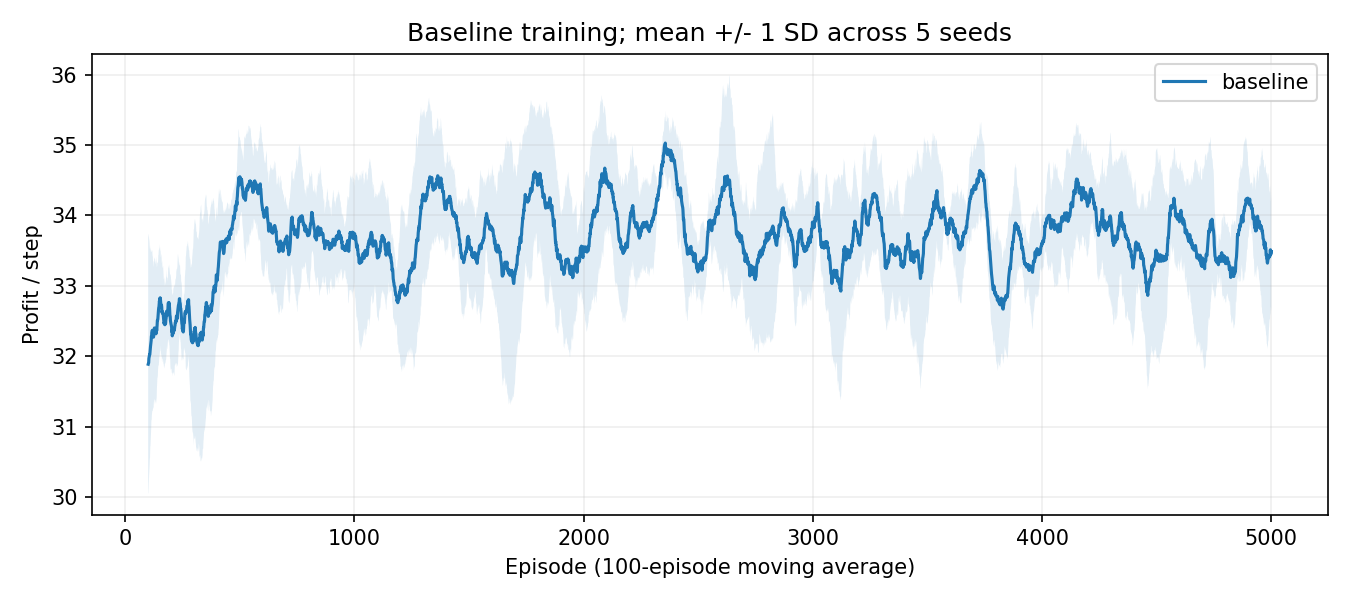
\includegraphics[width=0.98\linewidth]{results/assignment/learning_curve.png}
\captionof{figure}{Learning curve baseline: moving average 100 episode, mean và một SD qua năm seed.}
\end{center}

\begin{center}
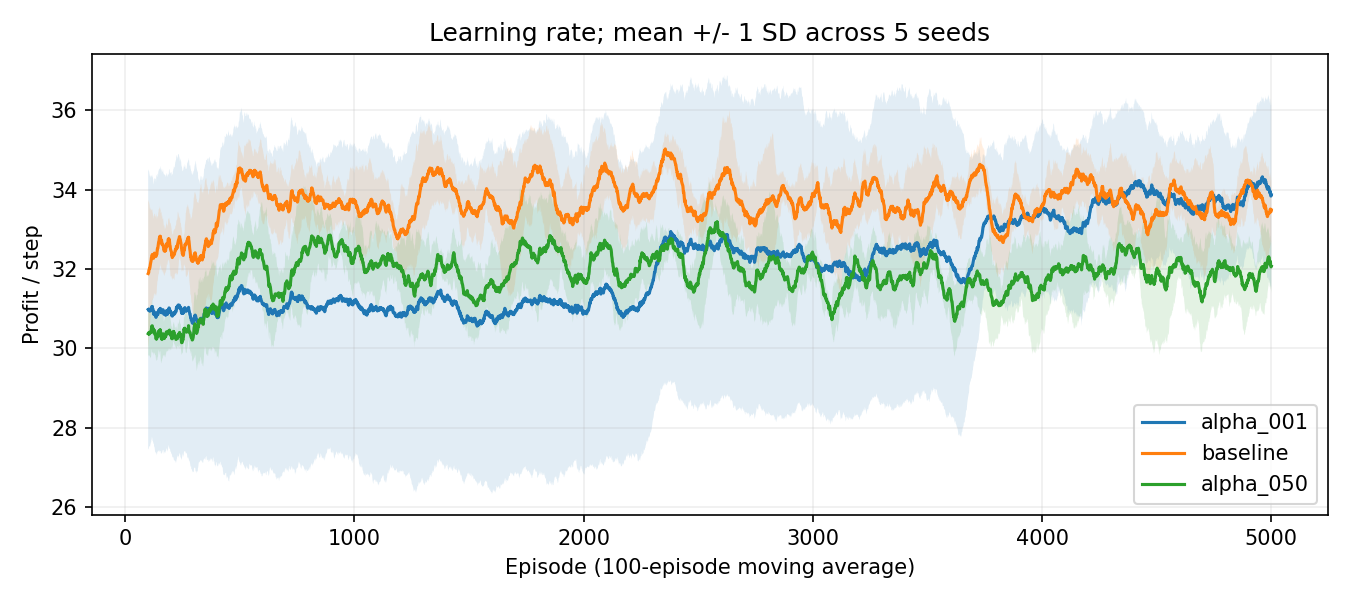
\includegraphics[width=0.98\linewidth]{results/assignment/learning_rates.png}
\captionof{figure}{So sánh ba learning rate với cùng epsilon schedule.}
\end{center}

\begin{center}
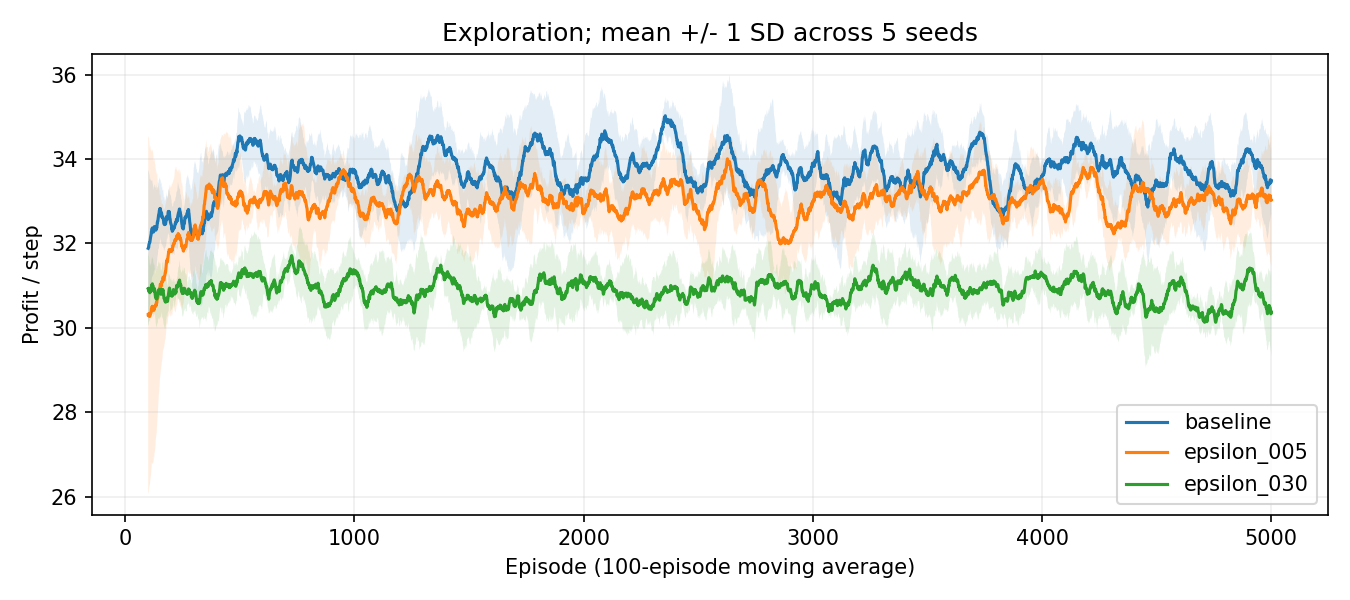
\includegraphics[width=0.98\linewidth]{results/assignment/exploration.png}
\captionof{figure}{So sánh ba cấu hình epsilon; mọi cấu hình đánh giá với epsilon bằng 0.}
\end{center}

\begin{center}
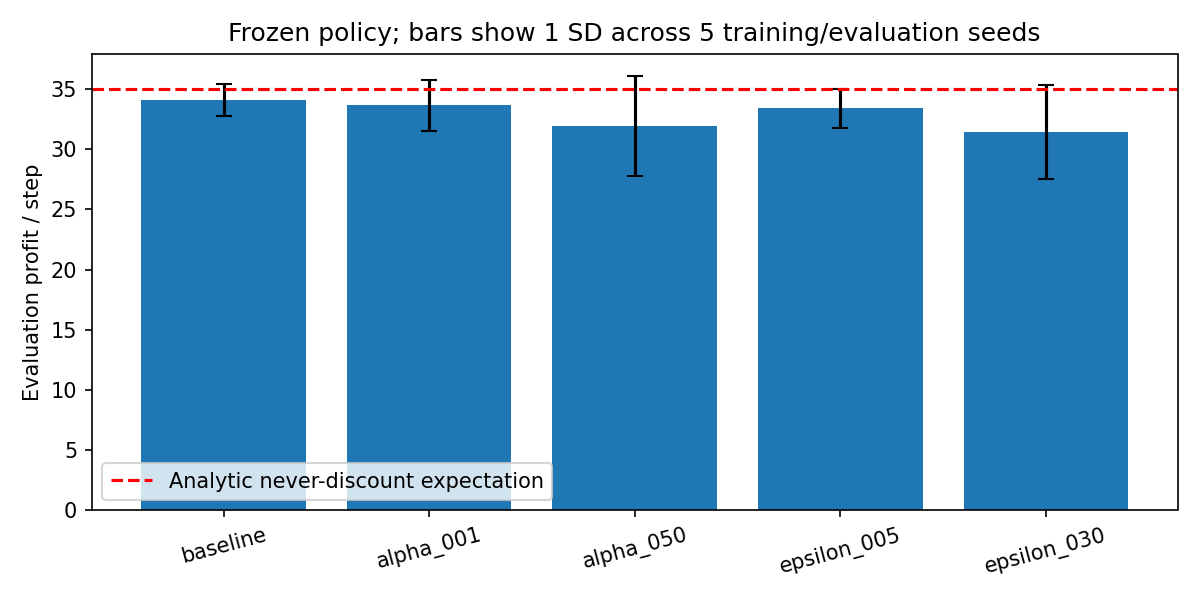
\includegraphics[width=0.98\linewidth]{results/assignment/evaluation.png}
\captionof{figure}{Policy đóng băng: mean và SD giữa seed; đường 35 là kỳ vọng lý thuyết.}
\end{center}

\begin{center}
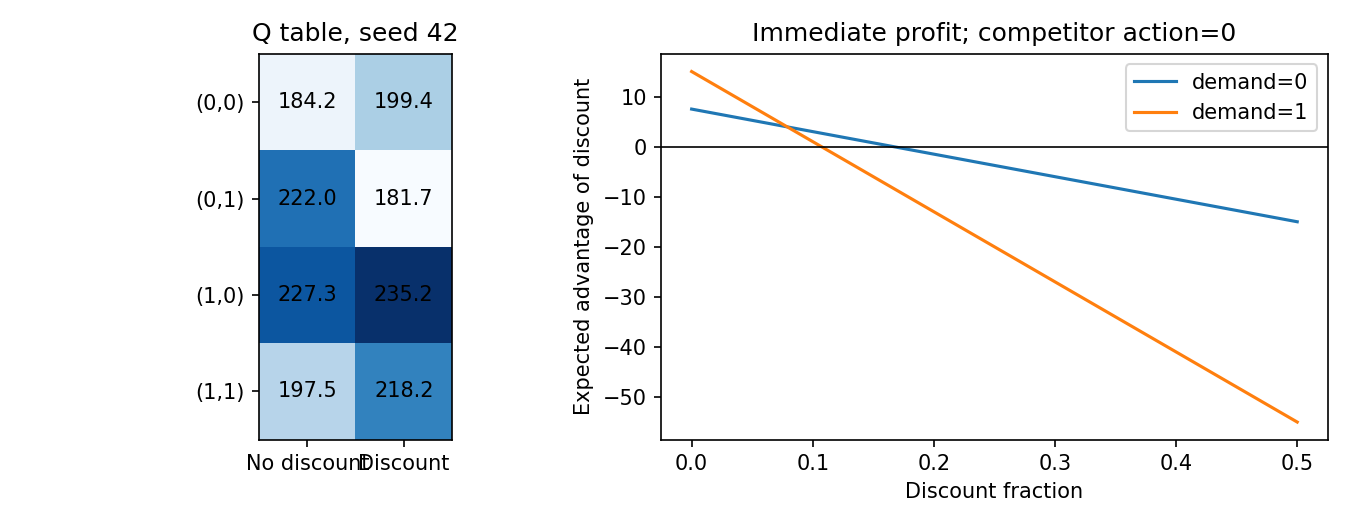
\includegraphics[width=0.98\linewidth]{results/assignment/q_and_sensitivity.png}
\captionof{figure}{Q-table seed 42 và độ nhạy lợi nhuận tức thời theo discount fraction.}
\end{center}

\subsection{Mã Python cốt lõi}\label{muxe3-python-cux1ed1t-luxf5i}

Đây là các đoạn mã được lấy trực tiếp từ nguồn đã thực thi. Tệp đầy đủ
và bản tham chiếu có trong thư mục assignment; các đoạn bên dưới đủ để
kiểm cách cập nhật, tách evaluation và tính oracle.

\lstinputlisting[firstline=60,lastline=73,caption={Q-learning và luật, trích từ mã chạy}]{assignment/agent02_experiment.py}
\lstinputlisting[firstline=106,lastline=118,caption={Quy hoạch động hữu hạn chân trời}]{assignment/agent02_experiment.py}
\lstinputlisting[firstline=120,lastline=149,caption={Đánh giá đóng băng với common random numbers}]{assignment/agent02_experiment.py}

\subsection{Bằng chứng kiểm
thử}\label{bux1eb1ng-chux1ee9ng-kiux1ec3m-thux1eed}

Bộ kiểm thử assignment có 12 ca, đã chạy thành công. Các ca kiểm công
thức ví dụ 4.65; terminal không bootstrap; observation sau joint action;
từ chối action sai; margin; bảng luật; Q không đổi khi đánh giá; tổng
action counts; tái lập evaluation; DP chọn không giảm; tái lập training;
và sample mean gần kỳ vọng 35 khi số episode lớn.

\begin{verbatim}
python3 -m unittest discover -s assignment -p 'test_*.py'
............
Ran 12 tests
OK
\end{verbatim}

Log thực tế được giữ trong build/assignment\_tests.log. Thời lượng đo cụ
thể phụ thuộc máy, nên không dùng thời lượng test làm chỉ số thuật toán.
Mười hai test không chứng nhận mô hình kinh tế đúng ngoài thực tế; chúng
kiểm những bất biến quan trọng của implementation.

\clearpage
\phantomsection\addcontentsline{toc}{section}{Tài liệu tham khảo}
\begin{thebibliography}{99}
\bibitem{slides} PGS.TS. Trần Đình Quế (tài liệu môn học được cung cấp), \emph{Developing Multiagent Systems: A Practical Tutorial with Python and PyTorch}, slide\_multiAgent\_system\_20.10.2026.pdf, 25 trang, 2026. Nguồn cục bộ trong đề bài.
\bibitem{lab} \emph{Laboratory Experiment 02: Reinforcement-Learning-Based Agents versus Rule-Based Agents}, Intelligent System Development, 2026--2027, assignment\_Agent02\_due\_29.10.pdf, 13 trang; agent02\_code.tex và agent02\_complementary\_code.pdf. Tài liệu cục bộ do người dùng cung cấp.
\bibitem{tran} K.-T. Tran, D. Dao, M.-D. Nguyen, Q.-V. Pham, B. O'Sullivan, H. D. Nguyen, \emph{Multi-Agent Collaboration Mechanisms: A Survey of LLMs}, arXiv:2501.06322v1, 10/01/2025. \url{https://arxiv.org/abs/2501.06322v1}. Phân tích trực tiếp bản PDF 35 trang được cung cấp.
\bibitem{naeem} M. Naeem, S. T. H. Rizvi, A. Coronato, \emph{A Gentle Introduction to Reinforcement Learning and Its Application in Different Fields}, IEEE Access, vol. 8, pp. 209320--209344, 2020. DOI: \href{https://doi.org/10.1109/ACCESS.2020.3038605}{10.1109/ACCESS.2020.3038605}. Phân tích trực tiếp bản PDF 25 trang được cung cấp.
\bibitem{sutton} R. S. Sutton, A. G. Barto, \emph{Reinforcement Learning: An Introduction}, 2nd ed., MIT Press, 2018. Tài liệu nền tảng được cả slide và paper RL dẫn chiếu.
\bibitem{watkins} C. J. C. H. Watkins, P. Dayan, \emph{Q-learning}, Machine Learning 8, 279--292, 1992. DOI: \href{https://doi.org/10.1007/BF00992698}{10.1007/BF00992698}.
\bibitem{autogen} Q. Wu et al., \emph{AutoGen: Enabling Next-Gen LLM Applications via Multi-Agent Conversation}, 2023. \url{https://arxiv.org/abs/2308.08155}.
\bibitem{metagpt} S. Hong et al., \emph{MetaGPT: Meta Programming for A Multi-Agent Collaborative Framework}, 2023, bản cập nhật 2024. \url{https://arxiv.org/abs/2308.00352}.
\bibitem{debate} Y. Du, S. Li, A. Torralba, J. B. Tenenbaum, I. Mordatch, \emph{Improving Factuality and Reasoning in Language Models through Multiagent Debate}, 2023. \url{https://arxiv.org/abs/2305.14325}.
\bibitem{torchce} PyTorch, \emph{CrossEntropyLoss}, tài liệu chính thức. \url{https://docs.pytorch.org/docs/stable/generated/torch.nn.CrossEntropyLoss.html}. Đối chiếu giao diện ngày 28/10/2026; môi trường thực nghiệm dùng PyTorch 2.8.0.
\bibitem{pythonasync} Python documentation, \emph{Coroutines and Tasks: asyncio.wait\_for}. \url{https://docs.python.org/3/library/asyncio-task.html}. Phần timeout được kiểm trực tiếp bằng tests trong môi trường thực thi.
\bibitem{artifacts} Bộ mã và dữ liệu tự thực thi của báo cáo: tutorial/, assignment/, results/, build/; seed và cấu hình lưu trong summary.json, intent\_metrics.json và mas\_metrics.json, ngày 28/10/2026. Đây là nguồn kết quả mô phỏng, không phải nguồn dữ liệu thị trường thực tế.
\end{thebibliography}

\end{document}
